%%%%%%%%%%%%%%%%%%%%%%%%%%%%%%%%%%%%%%%%%%%%%%%%%%%%%%%%%%%%
%% Chapter 3 — System Fundamentals and Problem Formulation
%% (10–15 pages)
%% Purpose: describe the physical and simulated system once,
%% define all coordinate spaces and interfaces, and formulate
%% the control objective mathematically.
%%%%%%%%%%%%%%%%%%%%%%%%%%%%%%%%%%%%%%%%%%%%%%%%%%%%%%%%%%%%
\chapter{System Fundamentals and Problem Formulation}
\label{chap:system}

Chapter~\ref{chap:fundamentals} established the control and modeling concepts
used in this thesis. This chapter converts that background into a fixed system
definition for the remaining work. It specifies the physical mechanism,
coordinate mappings, available measurements, actuator models, task geometry,
and evaluation interfaces before the controllers are compared. Keeping these
definitions together prevents later chapters from changing the plant,
observation set, or success criteria when interpreting results.

The physical machine and its two simulation representations are distinguished
explicitly. Simscape is the high-fidelity hydraulic source used for actuator
identification. IsaacLab/PhysX is the parallel environment used for policy
training, adaptation-data collection, and closed-loop evaluation. Both use the
cylinder ordering, kinematics, action contract, and cutter-tip task variables
defined here, but they are not assumed to be identical plants.

Sections~\ref{sec:sys:platform}--\ref{sec:sys:actuation} define the mechanism,
coordinate spaces, and signals. Sections~\ref{sec:sys:simscape} and
\ref{sec:sys:isaaclab} describe the two simulation models. The remaining
sections define the verge-following task, the R, IF, and AIF control stacks,
the control objective, and the acceptance gates used in the experiments.

\section{Manipulator Platform}
\label{sec:sys:platform}

The MULAG FME~500 is modeled as a serial-link mechanism with five
revolute joints. Four hydraulic
cylinders actuate the slew, two boom, and head-pivot joints. The
\emph{Messerkopf} rotation has no independent actuator and is locked at
the mowing configuration; it is therefore not a controlled degree of
freedom. The cylinder order used throughout the thesis is slew
(\emph{Drehzapfen}), boom~I (\emph{Ausleger~I}), boom~II
(\emph{Ausleger~II}), and head pivot (\emph{Messerkopf-Schwenk}).

Table~\ref{tab:sys:cylinders} gives the cylinder stroke ranges used in
the training data and the fixed limit of the \emph{Messerkopf} joint.
Task-space errors are measured at the cutter tip, which lies
$\unit[0.79]{m}$ below the \emph{Messerkopf} body origin.

\begin{table}[htbp]
  \centering
  \caption{Cylinder stroke ranges in the training data
  (Chapter~\ref{chap:data}) and the fixed \emph{Messerkopf} joint limit
  used for the mowing task.}
  \label{tab:sys:cylinders}
  \begin{tabular}{clcc}
    \toprule
    $i$ & Joint & Function & Limit \\
    \midrule
    1 & \emph{Drehzapfen}         & slew       & $0.018$--$0.493\,\mathrm{m}$ \\
    2 & \emph{Ausleger I}         & boom I     & $0.275$--$0.791\,\mathrm{m}$ \\
    3 & \emph{Ausleger II}        & boom II    & $0.309$--$0.857\,\mathrm{m}$ \\
    4 & \emph{Messerkopf-Schwenk} & head pivot & $0.269$--$0.689\,\mathrm{m}$ \\
    \midrule
    5 & \emph{Messerkopf}         & head rotation (locked) & $q_{5,\min}=q_{5,\max}=q_{5,\mathrm{lock}}$ \\
    \bottomrule
  \end{tabular}
\end{table}

Figure~\ref{fig:sys:topology} identifies the links, joints, and four actuator
channels used throughout the model.

\begin{figure}[htbp]
  \centering
  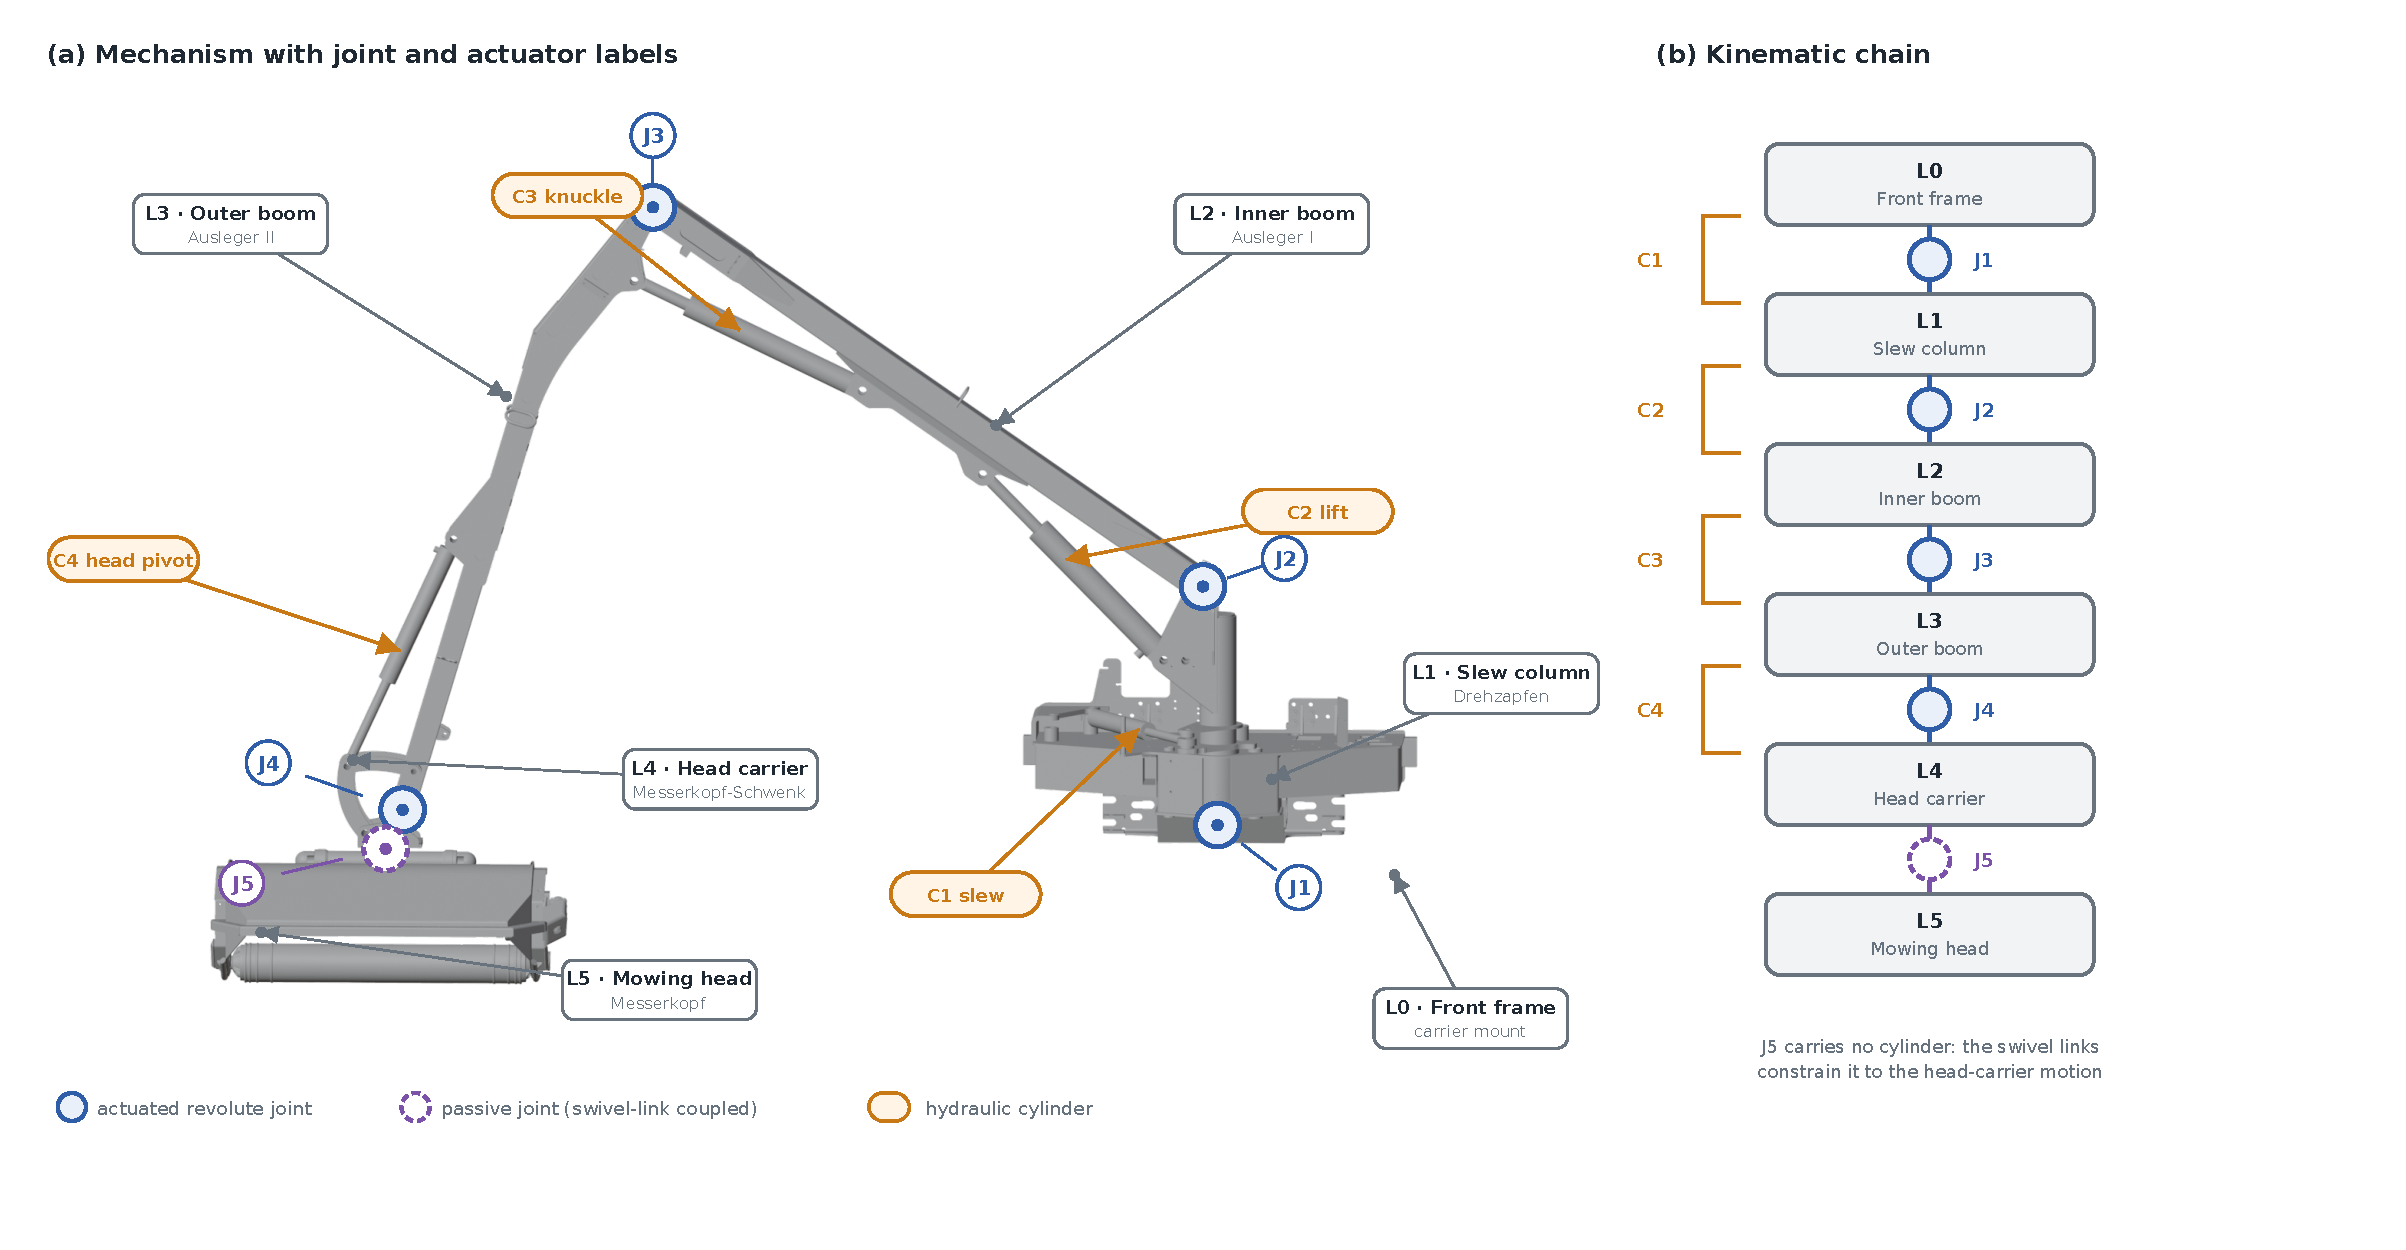
\includegraphics[width=\textwidth,trim=0 0 375 0,clip]{images/fme500_topology_annotated}
  \caption{Annotated CAD view of the MULAG FME~500. Links L0--L5,
  joints J1--J5, and the four hydraulic cylinders C1--C4 are identified;
  J5 denotes the \emph{Messerkopf} rotation, which is locked in the
  mowing configuration used in this thesis.}
  \label{fig:sys:topology}
\end{figure}

Figure~\ref{fig:sys:link-catalog} separates the rigid bodies that form the
assembled mechanism. The catalog makes the L0--L5 body assignment explicit
and shows the representative barrel--rod geometry used for cylinders C1--C4.

\begin{figure}[htbp]
  \centering
  \newcommand{\partcell}[4]{%
    \begin{minipage}[t]{.225\textwidth}
      \centering
      \textbf{\textcolor{#4}{#1}}\par
      \includegraphics[width=.96\linewidth]{images/links/#2}\par
      \vspace{-1mm}\small #3
    \end{minipage}}
  \partcell{L0}{link_frontrahmen}{Front frame}{cbblue}\hfill
  \partcell{L1}{link_drehzapfen}{Slew column}{cbblue}\hfill
  \partcell{L2}{link_ausleger_i}{Inner boom}{cbblue}\hfill
  \partcell{L3}{link_ausleger_ii}{Outer boom}{cbblue}

  \vspace{3mm}
  \makebox[\textwidth][c]{%
    \partcell{L4}{link_messerkopf_schwenk}{Head carrier}{cbblue}\hspace{.025\textwidth}%
    \partcell{L5}{link_messerkopf}{Mowing head}{cbblue}\hspace{.025\textwidth}%
    \partcell{C1--C4}{link_cylinder}{Double-acting cylinder}{cborange}}
  \caption{Individual CAD-derived bodies of the MULAG FME~500 shown at a
  common orthographic scale. L0--L5 are the front frame, slew column, inner
  boom, outer boom, head carrier, and mowing head. The C1--C4 panel shows the
  representative double-acting cylinder barrel--rod pair.}
  \label{fig:sys:link-catalog}
\end{figure}

Manufacturer CAD supplies the link geometry, joint locations, masses, centers
of mass, and inertia tensors through Phobos~\cite{vonszadkowski2020phobos}.
The same CAD-derived bodies and joint frames form the mechanical basis of the
Simscape and IsaacLab models, keeping dimensions, axes, masses, and cylinder
lever arms consistent while the hydraulic implementations remain
model-specific.

\section{Kinematic Structure and Coordinate Mappings}
\label{sec:sys:kinematics}

\subsection{Joint Space and Cylinder Space}

The configuration is $\bm{q} \in \mathbb{R}^5$; the actuated coordinates are
the four cylinder extensions $\bm{x} \in \mathbb{R}^4$. Cylinder $i$ joins CAD
attachment points $\bm{p}_A$ and $\bm{p}_B$ on adjacent links. Its length and
extension are
%
\begin{equation}
  \label{eq:sys:cyl-length}
  \ell_i(\bm{q}) = \bigl\| \bm{p}_B(\bm{q}) - \bm{p}_A(\bm{q}) \bigr\|,
  \qquad
  x_i = \ell_i(\bm{q}) - \ell_{0,i},
\end{equation}
%
with $\ell_{0,i}$ the retracted reference length. Differentiating
\eqref{eq:sys:cyl-length} gives the scalar mapping between joint motion
and extension rate,
%
\begin{equation}
  \label{eq:sys:cyl-jac}
  \dot{x}_i = J_{\mathrm{cyl},i}(\bm{q})\, \dot{\bm{q}},
  \qquad
  J_{\mathrm{cyl},i} = \bm{e}_i^{\!\top}
  \bigl( \bm{J}_B - \bm{J}_A \bigr),
\end{equation}
%
where $\bm{e}_i$ is the cylinder-axis unit vector and $\bm{J}_A$ and
$\bm{J}_B$ are attachment-point Jacobians. Virtual work gives
$\bm{\tau}_{\mathrm{act}}=\bm{J}_{\mathrm{cyl}}^{\top}\bm{F}_h$.
The mapping varies with configuration and stroke.

\subsection{Task Space and the Calibrated Cutter Jacobian}
\label{sec:sys:task-jacobian}

The cutter tip is expressed in the truck chassis frame
(\texttt{base\_link}); using the moving slew-base frame would corrupt the
tracking error. The controlled point includes the $\unit[-0.79]{m}$ tool-tip
offset. Vehicle motion supplies the along-track direction.

The calibrated Jacobian $\bm{J}_c\in\mathbb{R}^{3\times4}$ maps cylinder
extension rates to cutter-tip velocity. It was measured at the head-down
mowing pose by stepping each cylinder target and recording the settled cutter
displacement. Its singular values are $8.24$, $5.69$, and $2.79$, giving
rank~3. The damped least-squares controller in Chapter~\ref{chap:control}
uses this same Jacobian.

\section{Actuation and Measured State}
\label{sec:sys:actuation}

Table~\ref{tab:sys:signals} lists the signals and their availability.

\begin{table}[htbp]
  \centering
  \caption{Signal inventory of the modeled system. ``S'' marks signals
  present in the Simscape data exports, ``I'' signals available live in
  the IsaacLab environment, ``M'' quantities that exist there only
  through the learned models of Chapter~\ref{chap:models}, and ``P''
  \emph{privileged} quantities that exist in simulation but must never
  enter a deployable policy or estimator input.}
  \label{tab:sys:signals}
  \small
  \begin{tabular}{@{}llcl@{}}
    \toprule
    Signal & Dimension & Availability & Meaning \\
    \midrule
    $\bm{u}$ & $[-1,1]^4$ & S, M & normalized proportional-valve commands \\
    $\bm{x},\, \dot{\bm{x}}$ & $\mathbb{R}^4$ & S, I & cylinder extensions and velocities \\
    $\Delta\bm{p}$ & $\mathbb{R}^4$ & S, M & chamber pressure differences \\
    $\bm{F}$ & $\mathbb{R}^4$ & S & logged rod forces \\
    $\bm{q},\, \dot{\bm{q}}$ & $\mathbb{R}^5$ & S, I & joint positions and velocities \\
    $\bm{p}_c$ & $\mathbb{R}^3$ & S, I & cutter-tip position, truck frame \\
    $\bm{h}$ & $\mathbb{R}^{9}$ & I & forward terrain-height profile ahead of the cutter \\
    $\bm{c} = [\Delta\bm{x}^*, \Delta\dot{\bm{x}}^*]$ & $\mathbb{R}^8$ & I & desired cylinder command \\
    $\factorvec$ & $\mathbb{R}^6$ & P & physical randomization factors of the active plant \\
    $\bm{z} = \mu(\factorvec)$ & $\mathbb{R}^{d_z}$ & P & privileged dynamics latent, $d_z = 2$ \\
    $\latenthat$ & $\mathbb{R}^{d_z}$ & M & AAM estimate of $\bm{z}$ from observable history \\
    \bottomrule
  \end{tabular}
\end{table}

In IsaacLab, valve commands and differential pressures are learned-actuator
states, not direct measurements. R produces them internally; IF and AIF obtain
them from the inverse/forward pair. $\factorvec$ and
$\bm{z}=\mu(\factorvec)$ are privileged; only $\latenthat$ may enter AIF.

\subsection{Sensing and Observability}
\label{sec:sys:sensing}

The deployable observation contains articulation state, terrain rays, contact
signals, the desired cylinder command, and actuator-model pressure state. Plant
parameters are not observed; AIF infers their effect from causal history.

\begin{figure}[htbp]
  \centering
  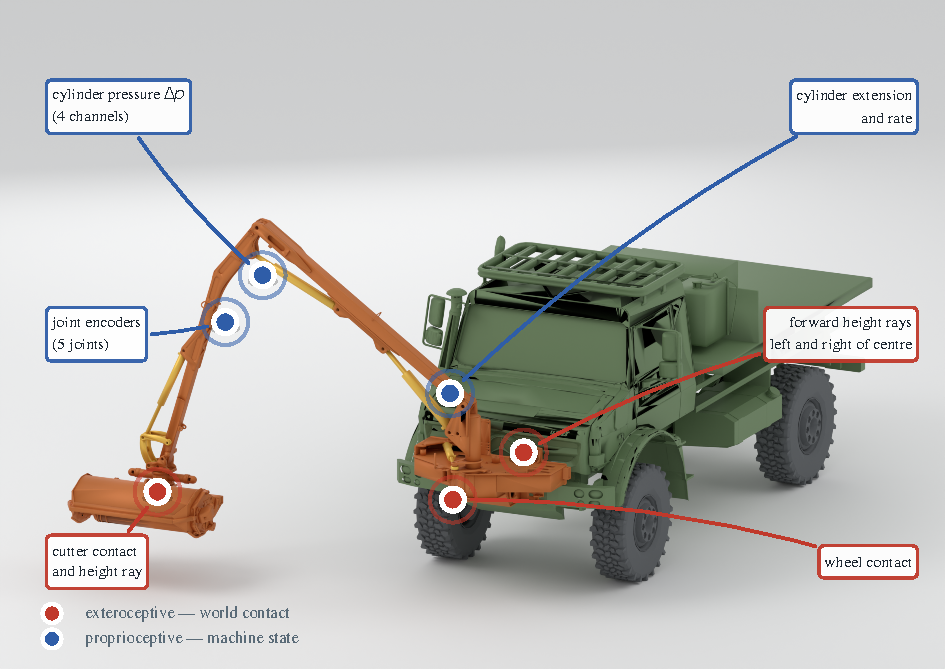
\includegraphics[width=.92\textwidth]{images/ch3_sensor_map}
  \caption{Sensor and observability map for the deployed
  controller. Blue callouts identify proprioceptive inputs: joint encoders,
  cylinder pressure differences, and cylinder extension and rate. Red
  callouts identify exteroceptive inputs: forward terrain-height rays and
  cutter and wheel contact.}
  \label{fig:sys:sensing}
\end{figure}

Figure~\ref{fig:sys:sensing} separates deployable measurements from
privileged plant information. Articulation state is read from the physics
engine without encoder noise or
quantisation.

\section{High-Fidelity Simscape Model}
\label{sec:sys:simscape}

The actuator models use a multi-domain Simscape model of the FME~500 developed
in the preceding master project. Table~\ref{tab:sys:provenance} distinguishes
the data source of each frozen component.

\begin{table}[htbp]
  \centering
  \caption{Provenance of each frozen actuator component. The command ROM
  is the only one that has been calibrated against the deployment plant;
  the inverse/forward pair is Simscape-identified throughout. This
  asymmetry is a property of the comparison and is carried into the
  discussion of Chapter~\ref{chap:evaluation}, not glossed over.}
  \label{tab:sys:provenance}
  \small
  \begin{tabular}{lp{4.4cm}p{5.0cm}}
    \toprule
    Component & Identified on & Calibrated on \\
    \midrule
    Command ROM & Simscape closed-loop export (grey-box, full model)
      & IsaacLab/PhysX closed-loop rollouts, via a bounded command-gated
        correction head only \\
    Control ID & Simscape closed-loop export & --- \\
    Strict FD & Simscape closed-loop export, retrained on the strict
        open-loop excitation export & --- \\
    $SD_0$, $\mu(\factorvec)$, $SD_z$, AAM
      & IsaacLab/PhysX adaptation collection (from scratch) & --- \\
    \bottomrule
  \end{tabular}
\end{table}

Simscape supplies the frozen ID and strict FD checkpoints. The ROM receives an
additional bounded IsaacLab calibration
(Section~\ref{sec:models:rom-calibration}). The adaptation models are trained
from IsaacLab data collected through the ROM and PhysX.

\subsection{The Command ROM as Deployment Actuator}
\label{sec:sys:rom-is-plant}

The command ROM plus PhysX is the deployment plant. Simscape is too slow for
policy training and bare PhysX has no hydraulics. The ROM is therefore both the
plant model and the actuator of R:

\begin{itemize}
  \item R uses the deployment plant itself and is the reference condition.
  \item IF replaces it with an independently identified inverse/forward pair.
  \item AIF adds online adaptation to IF.
\end{itemize}

The R--IF gap measures the transfer cost of the independently identified pair;
it is not a general ranking of the two model classes.

\subsection{Mechanical Subsystem}

The mechanism uses the CAD-derived links, joints, and cylinder attachment
frames of Section~\ref{sec:sys:platform}. It is simulated in Simscape
Multibody \cite{mathworks2024simscapemultibody}. The joint-space dynamics take
the standard manipulator form
%
\begin{equation}
  \label{eq:sys:eom}
  \bm{M}(\bm{q})\ddot{\bm{q}}
  + \bm{C}(\bm{q},\dot{\bm{q}})\dot{\bm{q}}
  + \bm{g}(\bm{q})
  + \bm{\tau}_{\mathrm{fric}}(\dot{\bm{q}})
  = \bm{\tau}_{\mathrm{act}} - \bm{J}^{\top}(\bm{q})\,\bm{F}_{\mathrm{ext}},
\end{equation}
%
with inertia $\bm{M}$ from the imported CAD. Friction combines viscous,
Coulomb, and Stribeck terms. The cutting load scales with feed velocity and
vegetation density. Each cylinder uses a
spherical--prismatic--cylindrical loop and hard stops enforce the limits in
Table~\ref{tab:sys:cylinders}.

\subsection{Hydraulic Subsystem}

Figure~\ref{fig:sys:schematic} shows four 4/3 valve-driven asymmetric cylinders
fed by a variable-speed, fixed-displacement pump
($Q_p=D_p\omega$), accumulator, and pressure-relief valve.

\begin{figure}[htbp]
  \centering
  \resizebox{\textwidth}{!}{%
  \begin{tikzpicture}[x=1cm,y=1cm,>=Latex,font=\footnotesize]
    \tikzset{hydchannel/.style={draw=cbblue!55!black,rounded corners=2pt,fill=cbblue!4,
      minimum width=8.35cm,minimum height=2.55cm}}
    % Reusable ISO-inspired cylinder and 4/3 directional-valve symbols.
    \newcommand{\hydcylinder}[1]{%
      \draw[thick,rounded corners=1pt,fill=black!2] (2.05,#1-.48) rectangle (4.65,#1+.48);
      \fill[cbblue!55] (2.12,#1-.41) rectangle (3.58,#1+.41);
      \fill[cbblue!32] (3.86,#1-.41) rectangle (4.58,#1+.41);
      \draw[thick,fill=black!48] (3.58,#1-.48) rectangle (3.86,#1+.48);
      \draw[thick,fill=black!38] (3.86,#1-.12) rectangle (5.25,#1+.12);
    }
    \newcommand{\dcvalve}[2]{%
      \draw[draw=cbblue!80!black,fill=white,thick] (6.00,#2-.42) rectangle (7.20,#2+.42);
      \draw[cbblue!80!black,thick] (6.40,#2-.42) -- (6.40,#2+.42);
      \draw[cbblue!80!black,thick] (6.80,#2-.42) -- (6.80,#2+.42);
      \draw[cbblue!80!black,semithick,-{Latex[length=1.2mm]}] (6.05,#2-.27) -- (6.35,#2+.27);
      \draw[cborange!90!black,semithick,-{Latex[length=1.2mm]}] (6.35,#2-.27) -- (6.05,#2+.27);
      \draw[black!55,semithick] (6.48,#2-.22) -- (6.72,#2+.22);
      \draw[black!55,semithick] (6.48,#2+.22) -- (6.72,#2-.22);
      \draw[cbblue!80!black,semithick,-{Latex[length=1.2mm]}] (6.85,#2+.27) -- (7.15,#2-.27);
      \draw[cborange!90!black,semithick,-{Latex[length=1.2mm]}] (7.15,#2+.27) -- (6.85,#2-.27);
      \draw[cbblue,semithick] (5.25,#2+.24) -- (6.00,#2+.24);
      \draw[cborange,semithick] (5.25,#2-.24) -- (6.00,#2-.24);
      \coordinate (v#1s) at (7.20,#2+.22);
      \coordinate (v#1t) at (7.20,#2-.22);
    }
    \node[font=\small\bfseries] at (4.1,.45) {Four independent actuator channels};
    \node[font=\small\bfseries] at (11.1,.45) {Shared hydraulic power unit};

    \node[hydchannel] at (4.1,-1.35) {};
    \node[hydchannel] at (4.1,-4.15) {};
    \node[hydchannel] at (4.1,-6.95) {};
    \node[hydchannel] at (4.1,-9.75) {};
    \draw[draw=cbblue!55!black,rounded corners=2pt,fill=cbblue!4] (9.45,.1) rectangle (12.8,-11.05);

    % Common supply and return rails
    \draw[cborange,very thick] (8.7,.08) -- (8.7,-10.55);
    \draw[cbblue,very thick] (8.98,.08) -- (8.98,-10.55);

    % C1
    \node[align=left,font=\small] at (1.22,-1.2) {C1\\\scriptsize Slew};
    \hydcylinder{-1.38}
    \dcvalve{1}{-1.38}
    \draw[cbblue,semithick] (v1s) -- (8.98,-1.16);
    \draw[cborange,semithick] (v1t) -- (8.7,-1.60);
    \node[font=\scriptsize,cbblue,fill=white,inner sep=1pt] at (5.60,-1.02) {$p_A$};
    \node[font=\scriptsize,cborange,fill=white,inner sep=1pt] at (5.60,-1.74) {$p_B$};

    % C2
    \node[align=left,font=\small] at (1.22,-4.0) {C2\\\scriptsize Boom I};
    \hydcylinder{-4.18}
    \dcvalve{2}{-4.18}
    \draw[cbblue,semithick] (v2s) -- (8.98,-3.96);
    \draw[cborange,semithick] (v2t) -- (8.7,-4.40);
    \node[font=\scriptsize,cbblue,fill=white,inner sep=1pt] at (5.60,-3.82) {$p_A$};
    \node[font=\scriptsize,cborange,fill=white,inner sep=1pt] at (5.60,-4.54) {$p_B$};

    % C3
    \node[align=left,font=\small] at (1.22,-6.8) {C3\\\scriptsize Boom II};
    \hydcylinder{-6.98}
    \dcvalve{3}{-6.98}
    \draw[cbblue,semithick] (v3s) -- (8.98,-6.76);
    \draw[cborange,semithick] (v3t) -- (8.7,-7.20);
    \node[font=\scriptsize,cbblue,fill=white,inner sep=1pt] at (5.60,-6.62) {$p_A$};
    \node[font=\scriptsize,cborange,fill=white,inner sep=1pt] at (5.60,-7.34) {$p_B$};

    % C4
    \node[align=left,font=\small] at (1.22,-9.6) {C4\\\scriptsize Head pivot};
    \hydcylinder{-9.78}
    \dcvalve{4}{-9.78}
    \draw[cbblue,semithick] (v4s) -- (8.98,-9.56);
    \draw[cborange,semithick] (v4t) -- (8.7,-10.00);
    \node[font=\scriptsize,cbblue,fill=white,inner sep=1pt] at (5.60,-9.42) {$p_A$};
    \node[font=\scriptsize,cborange,fill=white,inner sep=1pt] at (5.60,-10.14) {$p_B$};

    % Power unit
    \draw[thick,fill=cbblue!14] (10.15,-9.65) -- (10.15,-10.35) -- (12.1,-10.35) -- (12.1,-9.65);
    \draw[cbblue!80!black,very thick] (10.28,-9.88) -- (11.97,-9.88);
    \node[font=\scriptsize] at (11.12,-10.17) {reservoir};
    \draw[thick,fill=cbblue!12] (10.52,-8.65) -- (10.82,-8.35) -- (11.12,-8.65) -- (10.82,-8.95) -- cycle;
    \node[font=\scriptsize,anchor=west] at (11.38,-8.65) {filter};
    \draw[fill=cborange!45,thick] (10.82,-7.25) circle (.43);
    \node[font=\scriptsize] at (10.82,-7.25) {M};
    \draw[black!65,line width=1.2pt] (11.25,-7.25) -- (11.32,-7.25);
    \draw[fill=cbblue!40,thick] (11.75,-7.25) circle (.43);
    \fill[white] (11.60,-7.42) -- (11.60,-7.08) -- (11.98,-7.25) -- cycle;
    \node[font=\scriptsize] at (11.25,-6.5) {variable-speed pump};
    \draw[thick,rounded corners=6pt,fill=cbblue!35] (10.82,-5.42) rectangle (11.38,-4.38);
    \fill[cborange!55] (10.85,-5.37) rectangle (11.35,-4.92);
    \draw[thick] (10.82,-4.92) -- (11.38,-4.92);
    \node[font=\scriptsize] at (11.1,-5.65) {gas accumulator};
    \draw[thick,fill=white] (11.1,-3.25) circle (.32);
    \draw[cbblue,semithick] (11.1,-3.25) -- (11.25,-3.06);
    \node[font=\scriptsize] at (11.1,-3.85) {pressure sensor};
    \draw[thick,fill=cborange!22] (10.68,-1.9) rectangle (11.5,-1.15);
    \draw[->,semithick] (10.82,-1.75) -- (11.35,-1.3);
    \node[font=\scriptsize] at (11.1,-2.35) {relief valve};
    % The suction path is kept below the pump; the pressure path leaves from
    % the pump top. This avoids crossing the motor, pump, filter, and reservoir.
    \draw[black!65,semithick] (10.82,-9.65) -- (10.82,-8.95);
    \draw[black!65,semithick] (10.82,-8.35) -| (11.75,-7.68);
    \draw[cbblue,very thick] (11.75,-6.82) -- (11.75,-6.15);
    \draw[cbblue,very thick,-{Latex[length=1.8mm]}] (11.75,-6.15) -- (8.98,-6.15);
    \draw[cbblue,semithick] (8.98,-4.92) -- (10.82,-4.92);
    \draw[cbblue,semithick] (8.98,-3.25) -- (10.78,-3.25);
    \draw[cbblue,semithick] (8.98,-1.55) -- (10.68,-1.55);
    \draw[cborange,semithick] (11.50,-1.55) -- (12.35,-1.55) -- (12.35,-10.02) -- (12.1,-10.02);
    \draw[cborange,very thick,-{Latex[length=1.8mm]}]
      (8.7,-10.35) -- (8.7,-10.72) -- (9.75,-10.72) -- (9.75,-10.02) -- (10.15,-10.02);
  \end{tikzpicture}%
  }
  \caption{Hydraulic system schematic. Four proportional-valve cylinder
  channels share a variable-speed pump, reservoir, accumulator, sensor, and
  pressure-relief valve. Blue and orange rails denote supply and return.}
  \label{fig:sys:schematic}
\end{figure}

Figure~\ref{fig:sys:actuator-channel} identifies the cylinder chambers,
piston, seal, and rod used in the actuator model.

\begin{figure}[htbp]
  \centering
  \begin{tikzpicture}
    \node[inner sep=0] (cylinder) {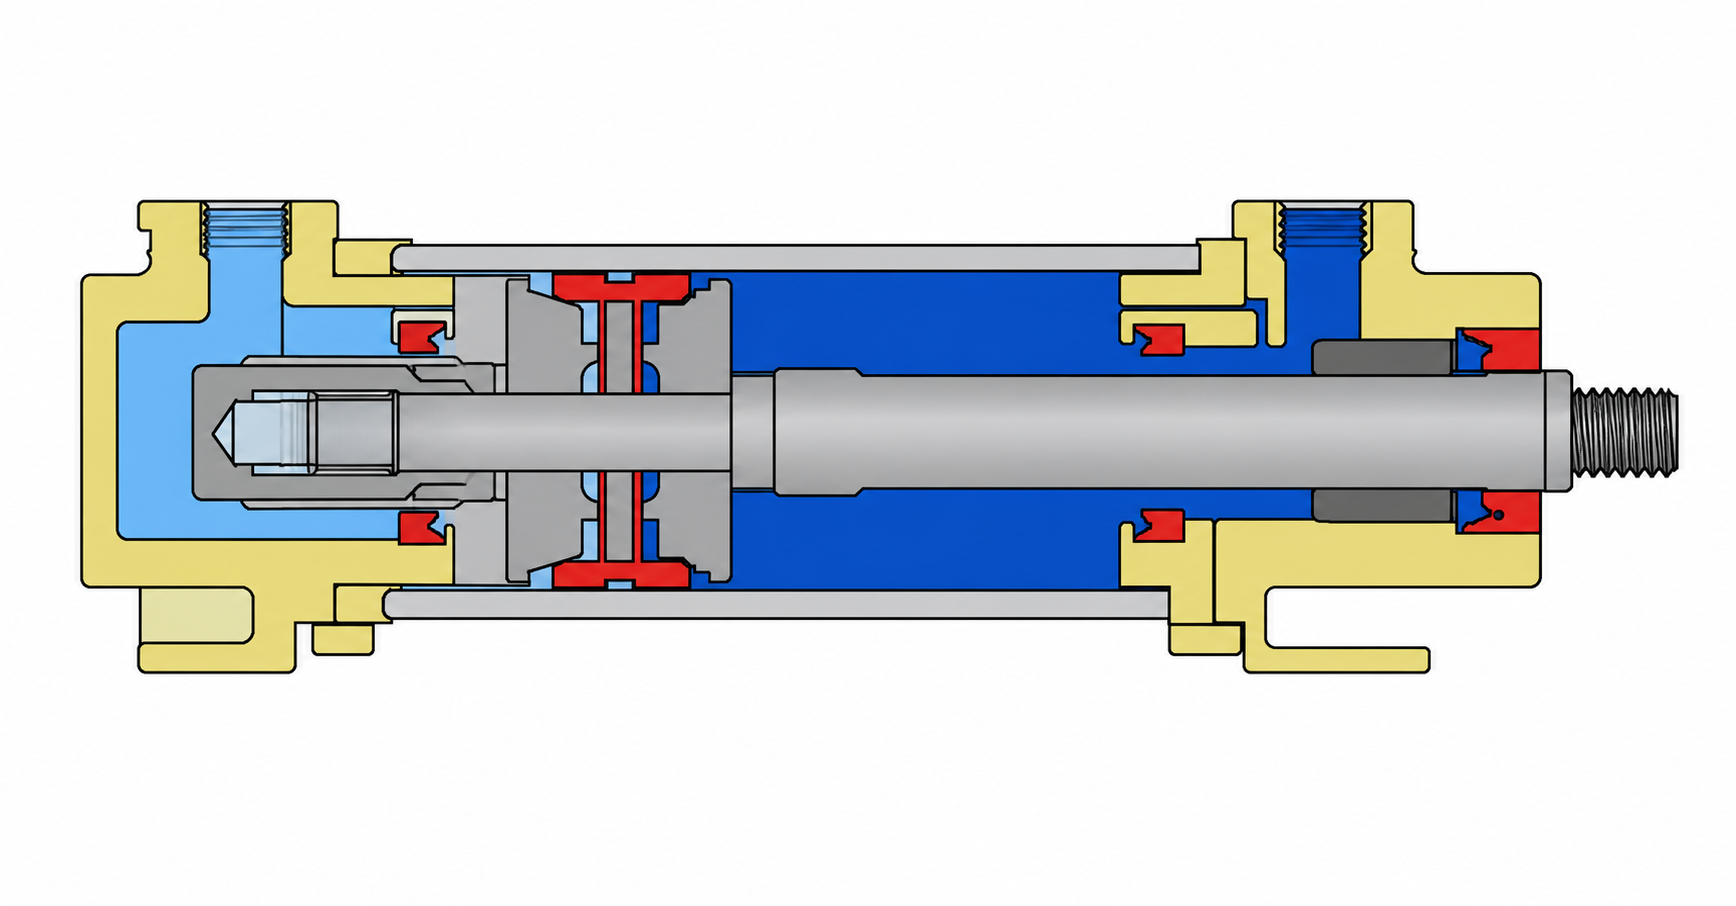
\includegraphics[width=.98\textwidth]{images/ch3_double_acting_cylinder_cutaway}};
    % Color-coded callouts follow the electrical--hydraulic--mechanical
    % annotation language used in Figure~\ref{fig:fund:chain}.
    \node[draw=cbblue,fill=white,rounded corners=1pt,inner sep=3pt,font=\normalsize,anchor=north west] (caplabel)
      at ([xshift=2mm,yshift=-2mm]cylinder.north west) {Cap-side chamber ($p_A,Q_A$)};
    \node[draw=cbgreen,fill=white,rounded corners=1pt,inner sep=3pt,font=\normalsize,anchor=north] (pistonlabel)
      at ([xshift=-18mm,yshift=-2mm]cylinder.north) {Piston};
    \node[draw=cbgreen,fill=white,rounded corners=1pt,inner sep=3pt,font=\normalsize,anchor=north] (seallabel)
      at ([xshift=12mm,yshift=-2mm]cylinder.north) {Piston seal};
    \node[draw=cbblue,fill=white,rounded corners=1pt,inner sep=3pt,font=\normalsize,anchor=north east] (rodlabel)
      at ([xshift=-2mm,yshift=-2mm]cylinder.north east) {Rod-side chamber ($p_B,Q_B$)};
    \node[draw=cbgreen,fill=white,rounded corners=1pt,inner sep=3pt,font=\normalsize,anchor=south east] (strokelabel)
      at ([xshift=-2mm,yshift=2mm]cylinder.south east) {Piston rod; stroke $x$};
    \draw[cbblue,semithick,-{Latex[length=1.8mm]}] (caplabel.south east) --
      ([xshift=15mm,yshift=-36mm]cylinder.north west);
    \draw[cbgreen,semithick,-{Latex[length=1.8mm]}] (pistonlabel.south) --
      ([xshift=-17mm,yshift=-42mm]cylinder.north);
    \draw[cbgreen,semithick,-{Latex[length=1.8mm]}] (seallabel.south) --
      ([xshift=-14mm,yshift=-26mm]cylinder.north);
    \draw[cbblue,semithick,-{Latex[length=1.8mm]}] (rodlabel.south west) --
      ([xshift=-60mm,yshift=-29mm]cylinder.north east);
    \draw[cbgreen,semithick,-{Latex[length=1.8mm]}] (strokelabel.north west) --
      ([xshift=-38mm,yshift=39mm]cylinder.south east);
  \end{tikzpicture}
  \caption{Annotated cutaway of an asymmetric double-acting hydraulic
  cylinder. The cap-side and rod-side chamber pressures generate the piston
  force and rod stroke.}
  \label{fig:sys:actuator-channel}
\end{figure}

The 4/3 valve in Figure~\ref{fig:sys:schematic} meters flow to the cylinder
chambers. The
chamber pressures follow
%
\begin{equation}
  \label{eq:sys:continuity}
  \dot{p}_1 = \frac{E_{\mathrm{eff}}}{V_1(x)}
    \bigl( Q_1 - A_1 \dot{x} - C_{\mathrm{leak}}(p_1 - p_2) \bigr),
  \qquad
  \dot{p}_2 = \frac{E_{\mathrm{eff}}}{V_2(x)}
    \bigl( -Q_2 + A_2 \dot{x} + C_{\mathrm{leak}}(p_1 - p_2) \bigr),
\end{equation}
%
where $V_{1,2}(x)$ include dead volumes, $A_1\neq A_2$, and
$C_{\mathrm{leak}}$ is internal leakage. Entrained air is represented by
%
\begin{equation}
  \label{eq:sys:bulk}
  E_{\mathrm{eff}}(p) =
  \left( \frac{1}{E_f} + \frac{\alpha}{p} \right)^{-1},
\end{equation}
%
Valve flow follows the orifice law of
Section~\ref{sec:fund:actuation-chain}; spool dynamics are
$\dot{x}_v=(u-x_v)/\tau_v$. The piston force is
$F_h=p_1A_1-p_2A_2-F_{\mathrm{fric}}(\dot{x})$. The coupled model is stiff and
uses a variable-step implicit solver, which prevents RL-time simulation.

\subsection{Validated Scope of the Model}
\label{sec:sys:simscape-validation}

Validation uses a fixed integral-backstepping controller at $\unit[0.01]{s}$
while sweeping $\beta\in\{0.5,1.0,1.5,2.0\}\,\mathrm{GPa}$. Slew-axis delay
falls from about $\unit[0.85]{s}$ to $\unit[0.65]{s}$, the system delay index
from $\unit[0.45]{s}$ to $\unit[0.35]{s}$, and task-space tracking error by
about 11\,\%. The improvement saturates beyond $\unit[1.5]{GPa}$.

The model represents one machine, omits thermal dynamics, and treats the logged
rod-force channel as unreliable after the piston-area consistency audit
(Section~\ref{sec:models:rom}). Chapter~\ref{chap:data} introduces variation
through parameter randomization.

\section{IsaacLab Environment}
\label{sec:sys:isaaclab}

Policy training, adaptation-data collection, and evaluation run in
IsaacLab~\cite{mittal2023orbit} on PhysX. The USD articulation contains the
Unimog carrier, five arm links, and four prismatic cylinder joints. Learned
actuator models supply the hydraulic behavior between the controller and PhysX
cylinder targets.

\subsection{Simulation and Control Rates}
\label{sec:sys:timing}

Table~\ref{tab:sys:rates} lists the four simulation clocks. PhysX runs at
$\unit[120]{Hz}$ and the policy at $\unit[60]{Hz}$. The learned actuator models
and AAM update every three policy steps ($\unit[0.05]{s}$); their prediction is
held across the intervening PhysX updates. Data collection uses this same
$\unit[50]{ms}$ grid.

\begin{table}[htbp]
  \centering
  \caption{The four rates of the simulated system. They are reported
  separately throughout the thesis; ``the control frequency'' is not a
  well-defined quantity here.}
  \label{tab:sys:rates}
  \small
  \begin{tabular}{lll}
    \toprule
    Layer & Step & Rate \\
    \midrule
    PhysX physics                & $\unit[1/120]{s}$   & $\unit[120]{Hz}$ \\
    Policy / control (decimation 2) & $\unit[1/60]{s}$ & $\unit[60]{Hz}$ \\
    Learned actuator model (3 control steps) & $\unit[0.05]{s}$ & $\unit[20]{Hz}$ \\
    AAM latent update            & $\unit[0.05]{s}$    & $\unit[20]{Hz}$ \\
    \bottomrule
  \end{tabular}
\end{table}

\subsection{Environment Configuration Details}

The arm root is spawned at $z=\unit[1.26]{m}$; ground-height spawning buries
the vehicle. Cylinder targets are integrated in reference space so gravity does
not erase commanded increments. Vehicle motion is scripted because the authored
tyres and suspension do not provide reliable PhysX traction; a planar fixture
holds lateral position and heading.

\section{The Verge-Following Task}
\label{sec:sys:task}

\subsection{Task Definition}

The task is moving verge following. The truck drives a $\unit[26]{m}$ strip at
a speed sampled from $2$ to $\unit[7]{km/h}$; development uses
$\unit[4]{km/h}$. Episodes allow $2808$ steps ($\unit[46.8]{s}$), while scoring
stops when the strip is completed. The arm must keep the cutter at the target
height, on the verge centre line, in contact with the ground, and within its
travel limits. Terrain height is randomized per environment
(Figure~\ref{fig:sys:verge-task-render}).

\begin{figure}[htbp]
  \centering
  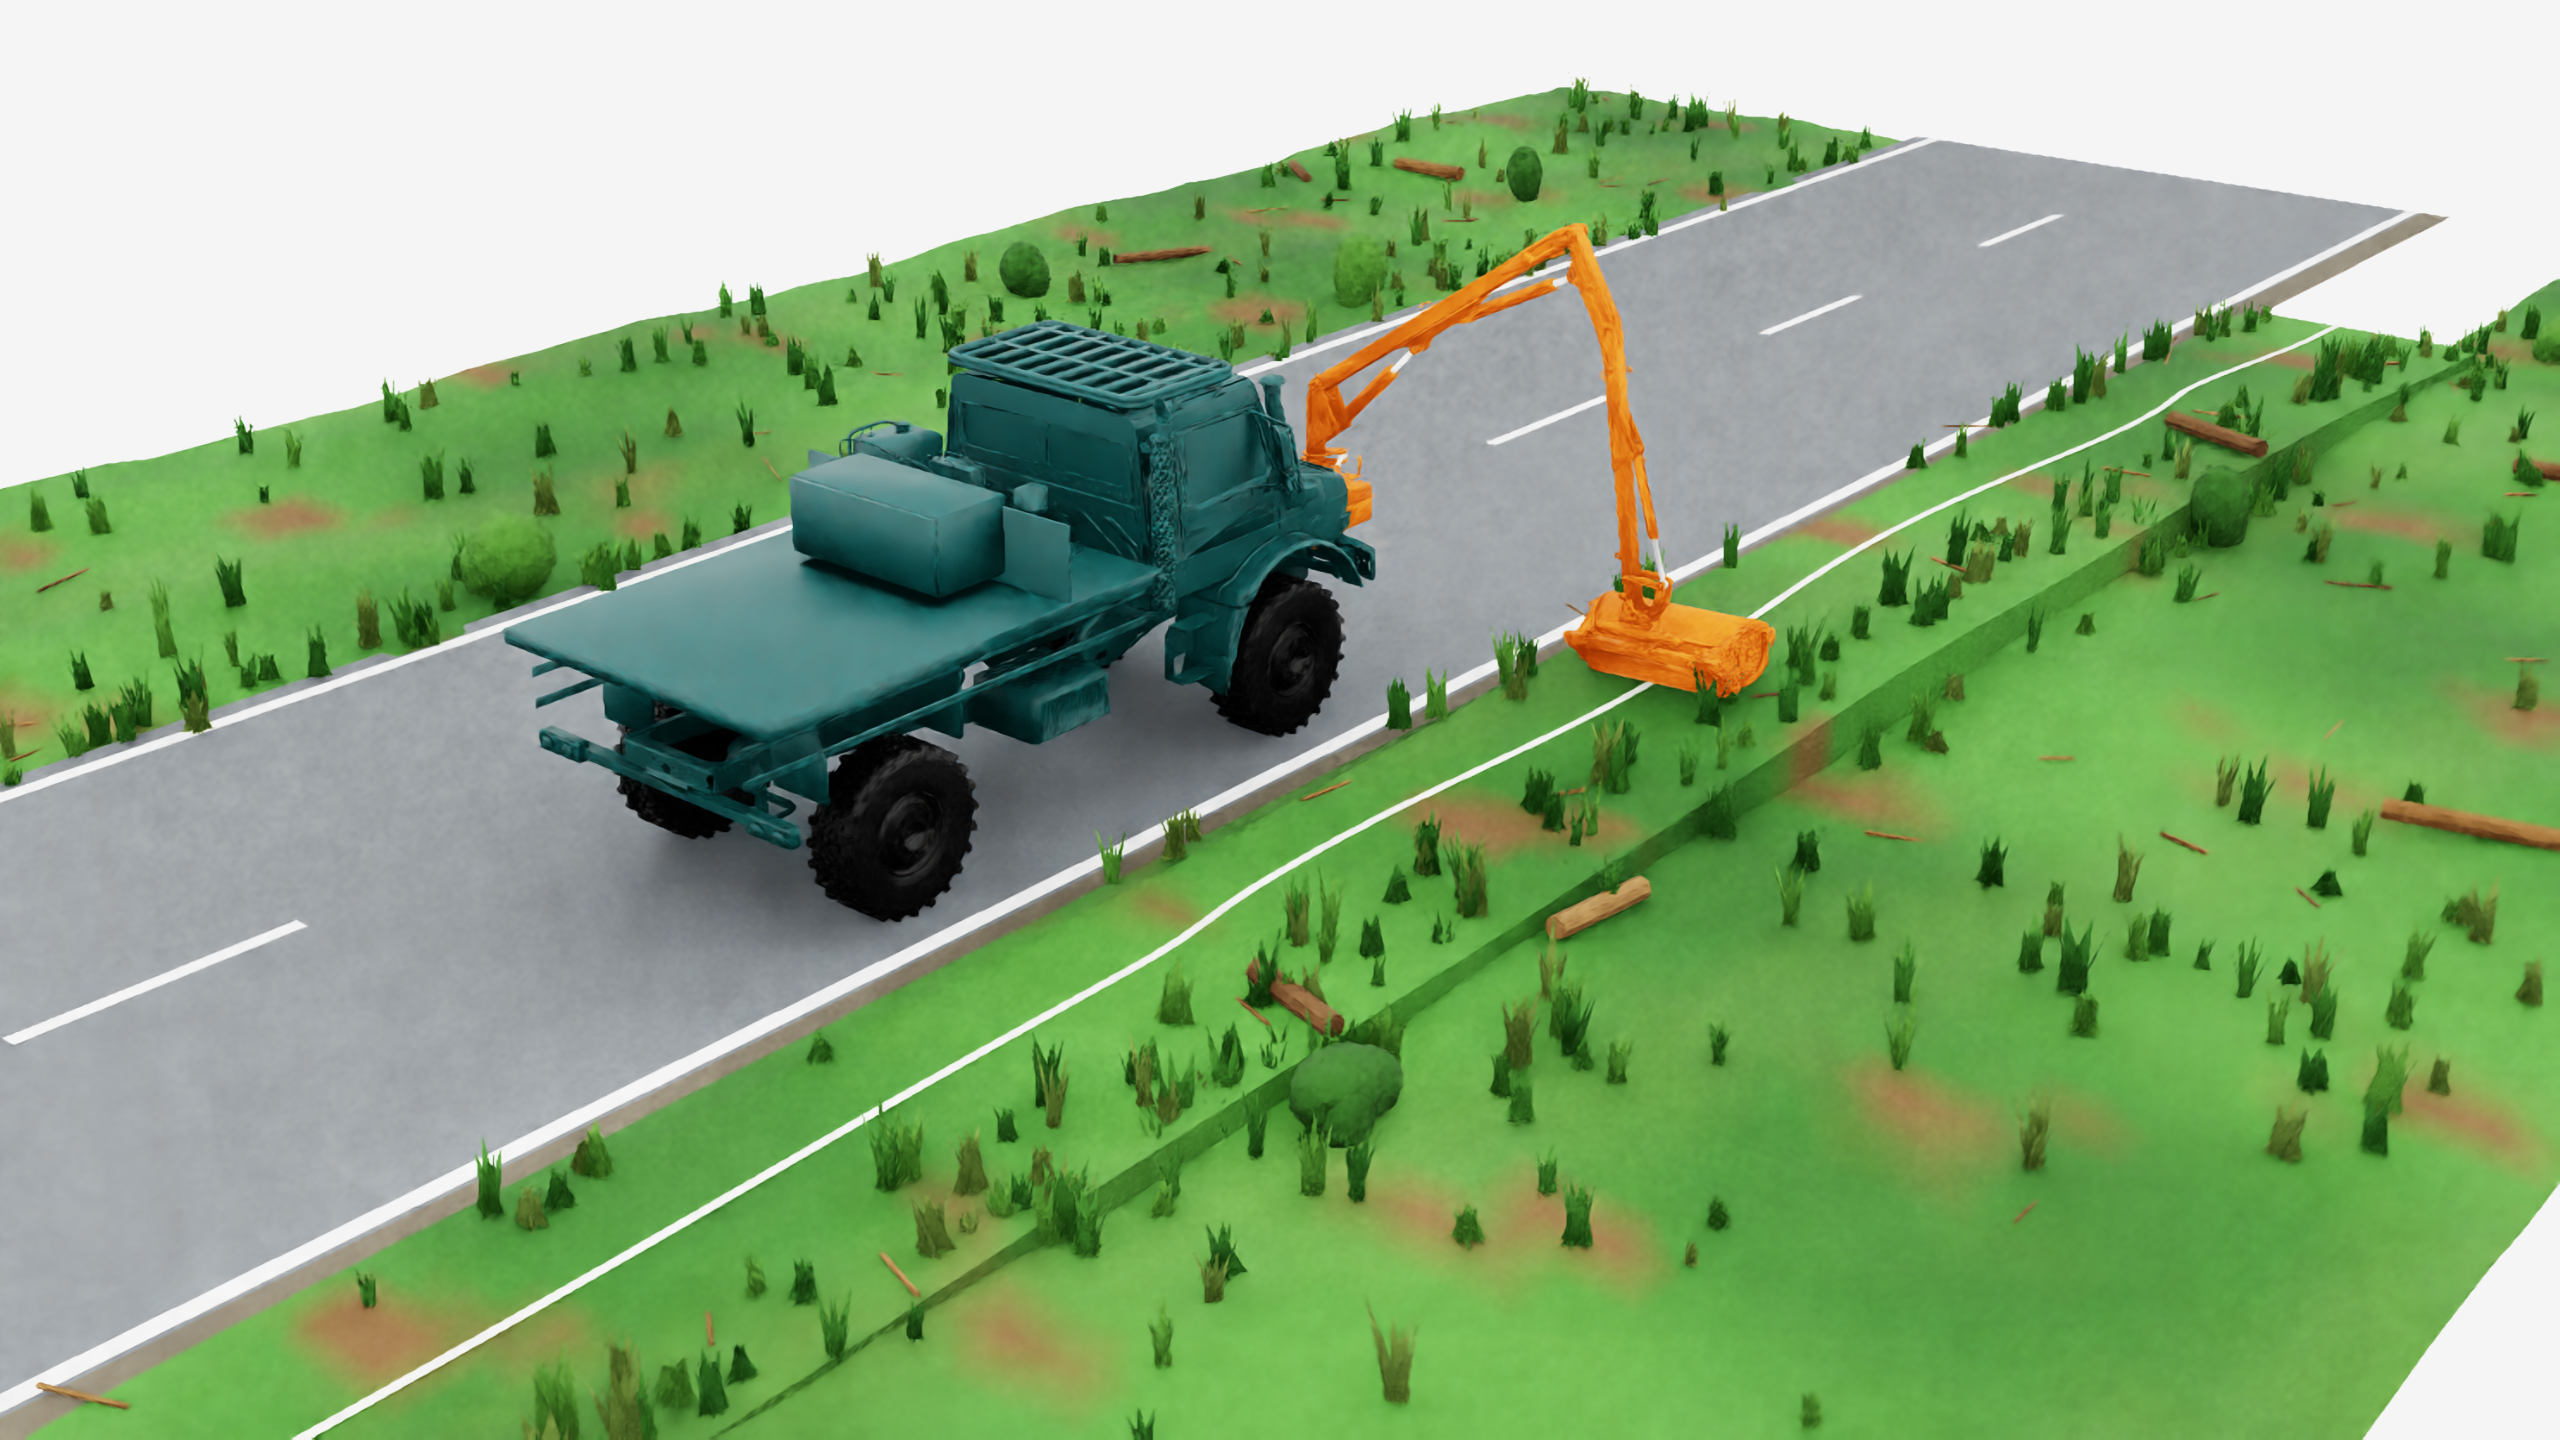
\includegraphics[width=\textwidth]{images/ch3_verge_task_render.png}
  \caption{IsaacLab realization of the moving verge-following task. The
  scripted truck travels on the level road while the four-cylinder arm places
  the cutter above the procedurally generated verge and follows the white
  reference path. Randomized grass, bushes, soil patches, twigs, and logs form
  a non-colliding visual layer; the underlying verge mesh supplies the terrain
  disturbance and height-sensing geometry used by the controller.}
  \label{fig:sys:verge-task-render}
\end{figure}

Eleven reference-path families span straight, periodic, spline, sweep, and
lane-change motion. Results use the worst path family and terrain mesh rather
than a pooled score. A regression test verifies that all eleven families are
distinct.

\subsection{Task Feasibility and Plant Capability}
\label{sec:sys:capability}

The action contract limits cylinders~1--3 to $\unit[4]{mm}$ per policy step,
which bounds lateral cutter speed at
%
\begin{equation}
  \label{eq:sys:rate-ceiling}
  v_{\mathrm{lat}}^{\max}
  = \frac{\unit[4]{mm}}{\unit[1/60]{s}} = \unit[0.240]{m/s}.
\end{equation}
%
This uses the $\unit[1/60]{s}$ policy interval. Early path settings exceeded
this limit; the worst case (\texttt{boom\_sweep}) required $3.7\times$ the
available rate. Path and terrain parameters are now derived from
\eqref{eq:sys:rate-ceiling}, and a preflight check rejects infeasible tasks.

\section{Control Architecture}
\label{sec:sys:architecture}

\begin{figure}[t]
  \centering
  \begin{tikzpicture}[x=1cm,y=1cm,>=Latex,font=\small]
    \node[draw=cbblue!90!black,line width=.8pt,rounded corners=2pt,fill=cbblue!42,
      minimum width=6.4cm,minimum height=1.25cm,align=center,font=\small] (obs) at (0,0)
      {observation\\[-1pt]\scriptsize state, terrain, reference};
    \node[draw=cbblue!95!black,line width=.8pt,rounded corners=2pt,fill=cbblue!82,text=white,
      minimum width=6.4cm,minimum height=1.25cm,align=center,font=\small\bfseries] (policy) at (0,-2.05)
      {policy $\pi_\theta$};
    \node[draw=cborange!90!black,line width=.8pt,rounded corners=2pt,fill=cborange!78,
      minimum width=6.4cm,minimum height=1.25cm,align=center,font=\small] (contract) at (0,-4.1)
      {action contract\\[-1pt]\scriptsize bounded cylinder increment $\Delta x^*$};

    \node[draw=cbblue!90!black,line width=.8pt,rounded corners=3pt,fill=cbblue!8,minimum width=6.4cm,
      minimum height=4.55cm] (path) at (0,-7.55) {};
    \node[font=\small\bfseries,text=cbblue!85!black] at (0,-5.9) {actuator path};
    \node[draw=cbblue!95!black,line width=.8pt,rounded corners=2pt,fill=cbblue!82,text=white,
      minimum width=5.25cm,minimum height=.78cm,font=\small\bfseries] at (0,-6.63) {R: ROM};
    \node[draw=cborange!95!black,line width=.8pt,rounded corners=2pt,fill=cborange!86,
      minimum width=5.25cm,minimum height=.78cm,font=\small\bfseries] at (0,-7.65)
      {IF: ID $\longrightarrow$ FD};
    \node[draw=cbgreen!90!black,line width=.8pt,rounded corners=2pt,fill=cbgreen!78,text=white,
      minimum width=5.25cm,minimum height=.78cm,font=\small\bfseries] at (0,-8.67)
      {AIF: AAM + IF};

    \node[draw=cbgreen!90!black,line width=.8pt,rounded corners=2pt,fill=cbgreen!68,text=white,
      minimum width=6.4cm,minimum height=1.35cm,align=center,font=\small\bfseries] (plant) at (0,-11.15)
      {PhysX plant\\[-1pt]\scriptsize arm, terrain, and contact};

    \draw[sigarrow,cbblue!90!black] (obs) -- (policy);
    \draw[sigarrow,cborange!90!black] (policy) -- (contract)
      node[midway,right,font=\scriptsize] {$\Delta x^*$};
    \draw[sigarrow,cborange!90!black] (contract) -- (path.north);
    \draw[sigarrow,cbgreen!80!black] (path.south) -- (plant);
    \draw[sigarrow,cbgreen!80!black] (plant.west) -| (-4.25,-11.15) |- (obs.west)
      node[pos=.55,left,font=\scriptsize,text=cbgreen!60!black] {measured state};
  \end{tikzpicture}
  \caption{Deployed control stack. The policy produces a bounded cylinder
  increment; R, IF, or AIF realizes it in the shared PhysX plant. Measured
  state closes the loop.}
  \label{fig:sys:architecture}
\end{figure}

The vehicle advances at the scripted speed and the reference generator supplies
the verge centre line and cut height. The policy maps normalized observations to
four desired cylinder increments; it has no runtime baseline controller. The
action contract bounds those increments. R uses the command ROM, IF the frozen
inverse/forward pair, and AIF adds the bounded adapter conditioned on
$\latenthat$. All paths set the same PhysX cylinder target. The DLS controller
is used only for teaching and identification.

\section{Problem Formulation}
\label{sec:sys:problem}

The reference is the verge centre line $y_{\mathrm{ref}}(t)$ and cut height
$h_{\mathrm{ref}}$, expressed in the truck frame. With cutter-tip position
$\bm{p}_c(t)$ and terrain height $g(\cdot)$, the scored errors are
%
\begin{equation}
  \label{eq:sys:error}
  e_{\mathrm{lat}}(t) = p_{c,y}(t) - y_{\mathrm{ref}}(t),
  \qquad
  e_{\mathrm{cut}}(t)
    = \bigl(p_{c,z}(t) - g(\bm{p}_c(t))\bigr) - h_{\mathrm{ref}} .
\end{equation}
%
The objective is to minimize the mean and tail of both errors across path
families and terrain while maintaining contact, head alignment, and smooth
motion. Learned models are evaluated on one-step and recursive cylinder
predictions. The stacks are tested across the randomized plant family; AIF is
compared with IF on held-out factors.

Constraints are cylinder limits and headroom
(Table~\ref{tab:sys:cylinders}), the action contract, checkpoint output limits,
and the head-down condition.

\section{System-Level Evaluation Criteria}
\label{sec:sys:evaluation-criteria}

Controllers and models are evaluated separately. Controller scores can hide
actuator-model errors through policy compensation.

The system-level criteria cover three aspects of operation. Cut-height and
lateral errors measure task accuracy. Contact, head alignment, impact rate,
and cutter acceleration describe tool--terrain interaction and motion quality.
Cylinder headroom and safety terminations check whether the task is completed
without driving the mechanism into its limits. The metrics are evaluated over
the scored part of each episode and are kept in physical units where possible.
This makes a failed gate traceable to a specific limitation rather than to a
single combined reward value.

\subsection{Eight-Gate Acceptance Contract}
\label{sec:sys:gates}

Table~\ref{tab:sys:gates} defines the system-level acceptance contract.

All controller stacks are evaluated with the same path, terrain, and
randomization conditions. A stack passes only when it satisfies every gate;
strong mean tracking cannot compensate for loss of contact, inadequate
cylinder headroom, excessive impacts, or safety terminations. Worst-case
aggregation prevents easy terrain or path cases from masking a local failure.
Mean absolute errors quantify sustained tracking performance, while the lower
and upper percentiles capture short alignment, clearance, or acceleration
events that a mean can hide. Contact and termination measures are reported as
fractions so that episodes of different completed length remain comparable.

\begin{table}[htbp]
  \centering
  \caption{Eight system-level acceptance gates. Each gate uses at least three
  terrain meshes and the worst mesh; tracking-critical gates also use the worst
  path family. $^{\dagger}$Hard impacts is a wear constraint.}
  \label{tab:sys:gates}
  \small
  \begin{tabular}{llll}
    \toprule
    Gate & Metric & Threshold & Aggregation \\
    \midrule
    Cut height        & mean $|e_{\mathrm{cut}}|$
                      & $\leq \unit[0.040]{m}$ & worst mesh \\
    Lateral tracking  & mean $|e_{\mathrm{lat}}|$
                      & $\leq \unit[0.300]{m}$ & worst mesh, worst family \\
    Ground contact    & contact fraction
                      & $\geq 0.700$ & worst mesh, worst family \\
    Head alignment    & p01 head-down alignment
                      & $\geq 0.900$ & worst mesh \\
    Hard impacts$^{\dagger}$ & hard-impact step fraction
                      & $\leq 0.350$ & worst mesh \\
    Tool acceleration & p95 cutter acceleration
                      & $\leq \unit[120]{m/s^2}$ & worst mesh \\
    Cylinder headroom & p01 travel margin
                      & $\geq \unit[0.005]{m}$ & worst mesh \\
    Safety terminations & termination rate
                      & $\leq 0.080$ & worst mesh \\
    \bottomrule
  \end{tabular}
\end{table}

\subsection{Cylinder and Model Checks}

Cylinder checks use fresh $\pm\unit[10]{mm}$ commands, coordinated
$\unit[80]{mm}$ motions, return error, and saturation. Model checks use
one-step and rollout accuracy, input ablation, and Jacobian conditioning
(Chapter~\ref{chap:models}). Chapter~\ref{chap:evaluation} reports these with
the acceptance contract. The small command checks local response and deadband;
the coordinated motion checks coupling between actuator channels. Return error
tests reversibility, and saturation checks whether the learned model respects
the command and stroke limits. These diagnostics are interpreted alongside the
system gates, not as substitutes for closed-loop task performance.

The system is now specified. The next chapter turns to the data the learned
models are built from.
